\section{Frontend}

\subsection{Technologies and libraries} \label{_feTechnologies}

\subsubsection{ReactJs}
Reactjs is an open-source, front end, JavaScript library for building user interfaces or UI components. It is maintained by Facebook and a community of individual developers and companies. React can be used as a base in the development of single-page or mobile applications. However, React is only concerned with state management and rendering that state to the DOM, so creating React applications usually requires the use of additional libraries for routing, as well as certain client-side functionality.

\begin{itemize}
    \item \textbf{Used Version:} 17.0.1
\end{itemize}

\subsubsection{NextJs}
Next.js is a back-end JavaScript framework for React applications, and it enables automatic server-side rendering (SSR). With Next.js you can develop web applications, mobile apps, desktop apps and progressive web apps: it is built on the principle of "Build once, run anywhere". It is a framework that requires no setup - it uses the filesystem as an API. It also has built-in support for TypeScript, which makes use of Babel. Other features of Next.js are automatic code splitting, automatic routing, hot code reloading (only modified code is reloaded) and static export (with one command it can export a static site).

\begin{itemize}
    \item \textbf{Used Version:} 10.0.6
\end{itemize}

\subsubsection{Typescript}
TypeScript is an open-source language which builds on JavaScript, one of the world’s most used tools, by adding static type definitions. Types provide a way to describe the shape of an object, providing better documentation, and allowing TypeScript to validate that your code is working correctly. Writing types can be optional in TypeScript, because type inference allows you to get a lot of power without writing additional code.

\begin{itemize}
    \item \textbf{Used Version:} 4.1.5
\end{itemize}

\subsubsection{Stripe}
Stripe simplifies and helps make all phases of the purchase and treasury process of a transaction smoother and more secure. Through the use of ad-hoc tools developed to manage payment flows, anti-fraud tools, a billing platform for businesses offering consumer services and subscription plans, and a dedicated app for marketplaces and platforms that activate multiple parties in the transaction.

\begin{itemize}
    \item \textbf{Used Version:} 8.137.0
\end{itemize}

\subsection{Architectural Overview} \label{_feArchitecture}

\begin{figure}[H]
    \centering
    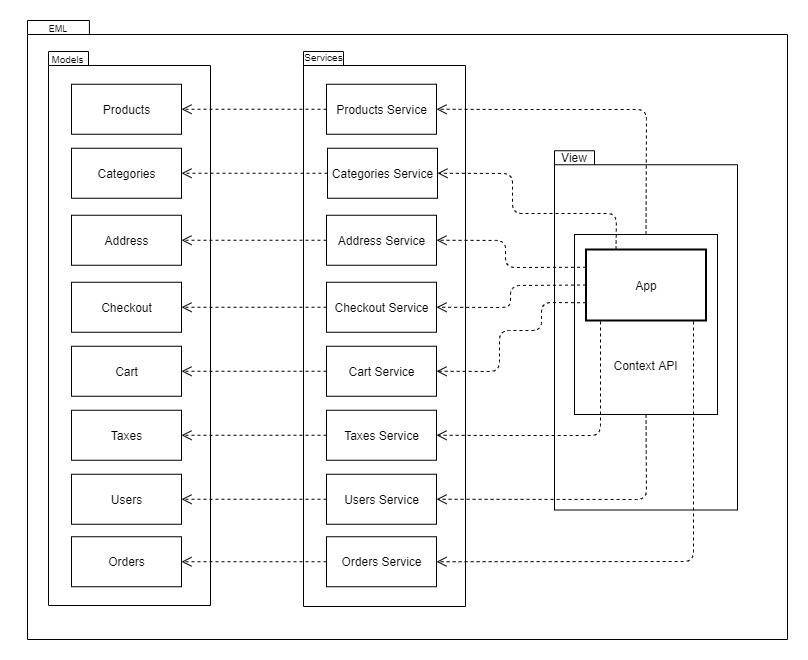
\includegraphics[width=0.9\textwidth]{res/images/frontend-diagrams/EML-FE.jpg}
    \caption{EML-FE architectural overview}
\end{figure}

The architecture designed to represent the project's UI consists of two fundamental parts that manage its data input and output. The frontend in the case of Emporio Lambda must only present the data coming from the Backend and allow the user to interact with the system quickly and efficiently.

The two fundamental parts that compose it are the services and the data persistence layer that provides a context to the application itself. Services are the connection point between the frontend and the backend, connecting the view to the various endpoints that can provide responses. Since the backend is developed with a microservices architecture, the frontend provides a particular service for each microservice available in the backend. This is designed to extend the software in case of additional maintenance later but also to easily detect any changes in the exposed microservices.

The data received from the endpoints and collected by the services is made available to the application. The received data can be used differently from each other allowing the application to have a persistence layer that can make all components in the hierarchy sharing the same data.

In a usual React/Next application, the common way of sharing data between two components is via prop drilling, i.e. passing the data as props from parent component to child component. The pop drilling method is suitable for a small application with two or three nested child components. However, for complicated applications, the data must be passed down as props to each of the levels until it reaches the desired component. This requires additional code. A way around this issue is to provide a global state that all components, regardless of their nested position, could access. This can be achieved using Redux, but with the release of React version 16.3, the new Context API was introduced as a solution to React prop drilling.

Context API is easy to is use as it has a short learning curve. It requires less code, and because there's no need of extra libraries, bundle sizes are reduced. Redux on the other hand requires adding more libraries to the application bundle. The syntax is complex and extensive creating unnecessary work and complexity.

For this reason, the group decided to implement data persistence through ContextAPI. This persistence layer is connected to the Authentication service and allows this data to be shared between the various pages of the UI.

\subsection{ContextAPI Overview} \label{_contextAPI}

\begin{figure}[H]
    \centering
    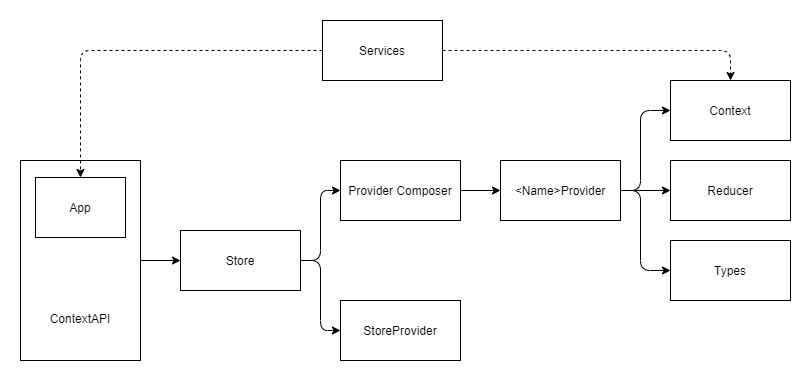
\includegraphics[width=0.9\textwidth]{res/images/frontend-diagrams/ContextAPI.png}
    \caption{ContextAPI overview}
\end{figure}

The ContextAPI shown in the figure defines in detail the operation of data persistence within the application. The ContextAPI consists of a Store that manages all the instances of the Providers that define a very particular application domain. Specifically, the Store consists of a StoreProvider, which provides the application with the data access point, and a ProviderComposer that combines the instances of the <Name>Provider in a single place then exposed to the UI by the StoreProvider.

The actual Provider that provide instances is, in the case of the application, the AuthProvider. It defines a particular instance that manages precise data such as authentication and session management for the User.



Specifically, a provider, such as the UserProvider, is made up of three fundamental parts:

\begin{itemize}
    \item \textbf{Context} where we find the persistent functions and data that are then made available to the application;
    \item \textbf{Reducer} a particular function responsible for changing data within the Context. The Reducer is the only way in which you can modify the Context data from the outside; 
    \item \textbf{Types} define actions with which the Reducer can go to modify the Context.
\end{itemize}

The fetching of the data as explained above is done by the Services which specifically provide the data either directly to the Context or to specific pages in the application.

\subsection{App Folder Structure Overview} \label{_folder}

\begin{figure}[H]
    \centering
    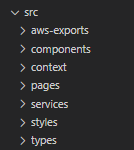
\includegraphics[width=10em]{res/images/frontend-diagrams/app-folder-structure.png}
    \caption{App folder structure overview for EML-FE}
\end{figure}

The structure of the application with regard to folders and the division of tasks follows the typical pattern of any React application. Let's see what it is made of:

\begin{itemize}
    \item \textbf{aws-exports} contains the definitions of variables for the use of AWS services;
    \item \textbf{components} contains all the reusable components of the application. Inside they are divided by scope and are accessible from all pages;
    \item \textbf{context} contains the definition of the single Context and the Store;
    \item \textbf{pages} represent the application url pages. Through Nextjs routing each of the defined pages creates a path reachable by the router;
    \item \textbf{services} manage all api requests. They are like a bridge or an adapter between the database server APIs and the persistance/view layer (pages and components) of our application. It will take care of all the network calls of our app.
    \item \textbf{styles} this module holds the application-level styles;
    \item \textbf{types} contains the definition of the types used by the application and coming from the Backend. Using Typescript to write the code, the types are a fundamental part for compilation.
\end{itemize}